\documentclass[11pt,border=8pt]{standalone}

\usepackage{fontspec}
\usepackage{array}
\setmainfont{TeX Gyre Termes}
\setsansfont{TeX Gyre Termes}
\newfontfamily\cjkfont{Noto Sans CJK SC}
\setmonofont{DejaVu Sans Mono}
\usepackage{tikz}
\usetikzlibrary{arrows.meta, calc, positioning, decorations.pathmorphing}

\definecolor{paperblue}{HTML}{2F6DA3}
\definecolor{topicorange}{HTML}{C77D28}
\definecolor{venueviolet}{HTML}{875A9A}
\definecolor{authorgreen}{HTML}{2E8B75}
\definecolor{softgray}{HTML}{4E5969}
\definecolor{signalred}{HTML}{C8553D}
\definecolor{ink}{HTML}{263238}
\definecolor{pale}{HTML}{FAFBFC}

\begin{document}
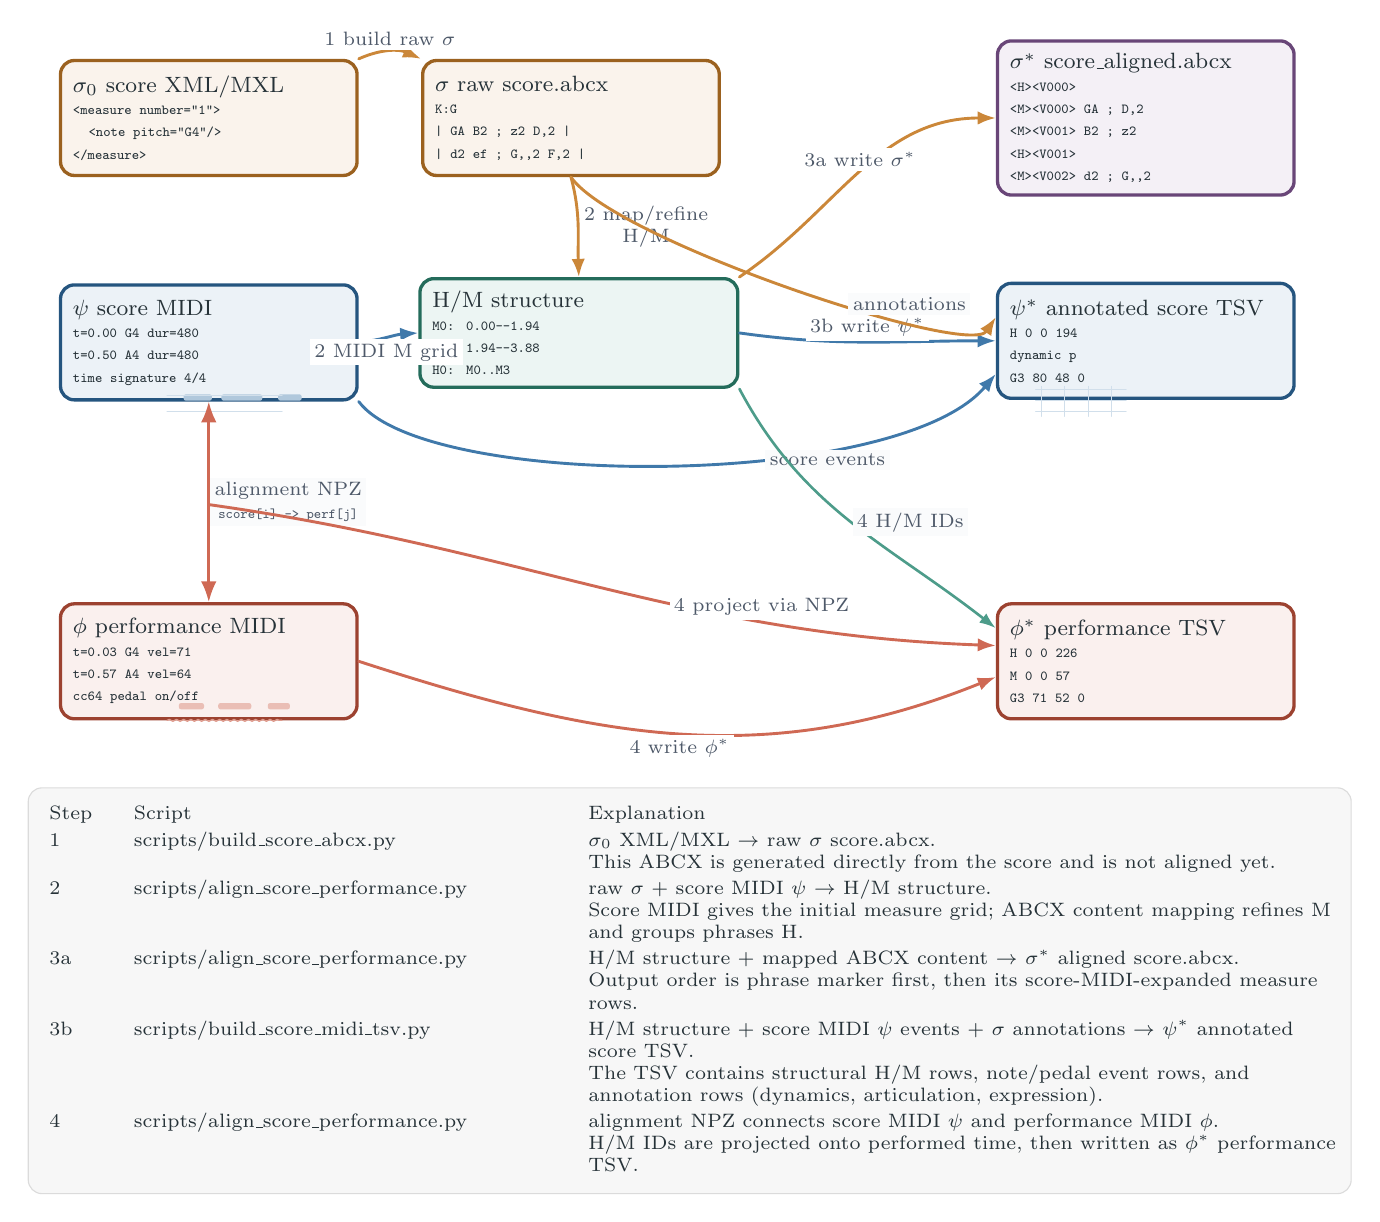
\begin{tikzpicture}[
    x=1cm,
    y=1cm,
    >=Latex,
    line cap=round,
    line join=round,
    every node/.style={font=\rmfamily, text=ink},
    card/.style={
        rounded corners=5pt,
        draw=#1!78!black,
        very thick,
        fill=#1!9,
        text width=3.45cm,
        minimum height=1.46cm,
        align=left,
        inner sep=4.5pt,
        font=\rmfamily\footnotesize
    },
    card/.default=paperblue,
    structcard/.style={
        rounded corners=5pt,
        draw=authorgreen!78!black,
        very thick,
        fill=authorgreen!9,
        text width=3.72cm,
        minimum height=1.20cm,
        align=left,
        inner sep=4.5pt,
        font=\rmfamily\footnotesize
    },
    edge/.style={-{Latex[length=2.2mm, width=1.6mm]}, line width=1.0pt, draw=softgray!90},
    sigmaedge/.style={-{Latex[length=2.3mm, width=1.7mm]}, line width=1.05pt, draw=topicorange!92},
    psiedge/.style={-{Latex[length=2.3mm, width=1.7mm]}, line width=1.05pt, draw=paperblue!92},
    phiedge/.style={-{Latex[length=2.3mm, width=1.7mm]}, line width=1.05pt, draw=signalred!88},
    label/.style={
        font=\rmfamily\scriptsize,
        fill=white,
        inner sep=1.6pt,
        text=softgray,
        align=center
    },
    tag/.style={
        rounded corners=4pt,
        fill=black!4,
        draw=black!14,
        inner sep=2pt,
        font=\rmfamily\tiny,
        text=softgray
    },
    mini/.style={font=\ttfamily\tiny, text=softgray},
    explain/.style={
        rounded corners=5pt,
        draw=black!14,
        fill=black!3,
        text width=16.45cm,
        align=left,
        inner sep=5pt,
        font=\rmfamily\scriptsize,
        text=ink
    }
]

% Concrete files / data objects.
\node[card=topicorange] (xml) at (2.35,6.55)
{{$\sigma_0$ score XML/MXL}\\[-0.5mm]
{\ttfamily\tiny <measure number="1">}\\[-0.5mm]
{\ttfamily\tiny \ \ <note pitch="G4"/>}\\[-0.5mm]
{\ttfamily\tiny </measure>}};

\node[card=topicorange] (abcx) at (6.95,6.55)
{{$\sigma$ raw score.abcx}\\[-0.5mm]
{\ttfamily\tiny K:G}\\[-0.5mm]
{\ttfamily\tiny | GA B2 ; z2 D,2 |}\\[-0.5mm]
{\ttfamily\tiny | d2 ef ; G,,2 F,2 |}};

\node[card=paperblue] (smidi) at (2.35,3.70)
{{$\psi$ score MIDI}\\[-0.5mm]
{\ttfamily\tiny t=0.00 G4 dur=480}\\[-0.5mm]
{\ttfamily\tiny t=0.50 A4 dur=480}\\[-0.5mm]
{\ttfamily\tiny time signature 4/4}};

\node[structcard] (hm) at (7.05,3.82)
{H/M structure\\[-0.5mm]
{\ttfamily\tiny M0: 0.00--1.94}\\[-0.5mm]
{\ttfamily\tiny M1: 1.94--3.88}\\[-0.5mm]
{\ttfamily\tiny H0: M0..M3}};

\node[card=venueviolet] (aligned) at (14.25,6.55)
{{$\sigma^\ast$ score\_aligned.abcx}\\[-0.5mm]
{\ttfamily\tiny <H><V000>}\\[-0.5mm]
{\ttfamily\tiny <M><V000> GA ; D,2}\\[-0.5mm]
{\ttfamily\tiny <M><V001> B2 ; z2}\\[-0.5mm]
{\ttfamily\tiny <H><V001>}\\[-0.5mm]
{\ttfamily\tiny <M><V002> d2 ; G,,2}};

\node[card=paperblue] (stsv) at (14.25,3.72)
{{$\psi^\ast$ annotated score TSV}\\[-0.5mm]
{\ttfamily\tiny H 0 0 194}\\[-0.5mm]
{\ttfamily\tiny dynamic p}\\[-0.5mm]
{\ttfamily\tiny G3 80 48 0}};

\node[card=signalred] (pmidi) at (2.35,-0.35)
{{$\phi$ performance MIDI}\\[-0.5mm]
{\ttfamily\tiny t=0.03 G4 vel=71}\\[-0.5mm]
{\ttfamily\tiny t=0.57 A4 vel=64}\\[-0.5mm]
{\ttfamily\tiny cc64 pedal on/off}};

\node[card=signalred] (ptsv) at (14.25,-0.35)
{{$\phi^\ast$ performance TSV}\\[-0.5mm]
{\ttfamily\tiny H 0 0 226}\\[-0.5mm]
{\ttfamily\tiny M 0 0 57}\\[-0.5mm]
{\ttfamily\tiny G3 71 52 0}};
\coordinate (npzrel) at (2.35,1.64);

% Small concrete visual motifs inside / around nodes.
\foreach \xx/\ww in {3.28/0.36,3.76/0.52,4.48/0.30} {
    \fill[paperblue!38, rounded corners=0.8pt] ({\xx-1.25},2.96) rectangle ++(\ww,0.08);
}
\draw[paperblue!22] (1.82,2.82) -- (3.28,2.82);
\draw[paperblue!22] (1.82,3.02) -- (3.28,3.02);

\foreach \xx/\ww in {3.22/0.32,3.72/0.42,4.35/0.28} {
    \fill[signalred!38, rounded corners=0.8pt] ({\xx-1.25},-0.96) rectangle ++(\ww,0.08);
}
\draw[decorate, decoration={snake, amplitude=0.35pt, segment length=2.6pt}, signalred!60, line width=0.45pt]
    (1.82,-1.10) -- (3.28,-1.10);

\foreach \xx in {12.92,13.22,13.52,13.82} {
    \draw[paperblue!22] (\xx,2.76) -- (\xx,3.14);
}
\foreach \yy in {2.82,2.96,3.10} {
    \draw[paperblue!22] (12.85,\yy) -- (14.00,\yy);
}

% Arrows: each path has its own channel and avoids nodes.
\draw[sigmaedge] (xml.north east) to[out=24,in=156]
    node[label, above] {1 build raw $\sigma$} (abcx.north west);

\draw[psiedge] (smidi.east) to[out=6,in=184]
    node[label, below, pos=0.46] {2 MIDI M grid} (hm.west);
\draw[sigmaedge] (abcx.south) to[out=-75,in=92]
    node[label, right] {2 map/refine\\H/M} (hm.north);

\draw[sigmaedge] (hm.north east) to[out=34,in=180]
    node[label, above] {3a write $\sigma^\ast$} (aligned.west);
\draw[psiedge] (hm.east) to[out=-8,in=180]
    node[label, above] {3b write $\psi^\ast$} (stsv.west);
\draw[psiedge] (smidi.south east) .. controls (5.10,1.82) and (11.10,1.82) ..
    node[label, fill=pale, below, pos=0.70] {score events} ($(stsv.west)+(0,-0.42)$);
\draw[sigmaedge] (abcx.south) .. controls (7.50,5.00) and (12.00,3.50) ..
    node[label, fill=pale, right, pos=0.60] {annotations} ($(stsv.west)+(0,0.30)$);

\draw[<->, line width=1.0pt, draw=signalred!88] (smidi.south) --
    node[label, fill=pale, right] {alignment NPZ\\{\ttfamily\tiny score[i] -> perf[j]}} (pmidi.north);
\draw[phiedge] (npzrel) to[out=-8,in=178]
    node[label, above, pos=0.72] {4 project via NPZ} ($(ptsv.west)+(0,0.20)$);
\draw[phiedge] (pmidi.east) to[out=-18,in=202]
    node[label, below] {4 write $\phi^\ast$} ($(ptsv.west)+(0,-0.20)$);
\draw[authorgreen!85, -{Latex[length=2.1mm, width=1.5mm]}, line width=0.95pt]
    (hm.south east) to[out=-62,in=142]
    node[label, fill=pale, right] {4 H/M IDs} ($(ptsv.west)+(0,0.42)$);

% Step explanation.
\node[explain, anchor=north west] at (0.05,-1.95)
{\renewcommand{\arraystretch}{1.18}
\scriptsize
\begin{tabular}{@{}>{\raggedright\arraybackslash}p{0.65cm}>{\raggedright\arraybackslash}p{5.35cm}>{\raggedright\arraybackslash}p{9.65cm}@{}}
Step & Script & Explanation\\
1 & scripts/build\_score\_abcx.py
& $\sigma_0$ XML/MXL $\rightarrow$ raw $\sigma$ score.abcx.\newline
This ABCX is generated directly from the score and is not aligned yet.\\
2 & scripts/align\_score\_performance.py
& raw $\sigma$ + score MIDI $\psi$ $\rightarrow$ H/M structure.\newline
Score MIDI gives the initial measure grid; ABCX content mapping refines M and groups phrases H.\\
3a & scripts/align\_score\_performance.py
& H/M structure + mapped ABCX content $\rightarrow$ $\sigma^\ast$ aligned score.abcx.\newline
Output order is phrase marker first, then its score-MIDI-expanded measure rows.\\
3b & scripts/build\_score\_midi\_tsv.py
& H/M structure + score MIDI $\psi$ events + $\sigma$ annotations $\rightarrow$ $\psi^\ast$ annotated score TSV.\newline
The TSV contains structural H/M rows, note/pedal event rows, and annotation rows (dynamics, articulation, expression).\\
4 & scripts/align\_score\_performance.py
& alignment NPZ connects score MIDI $\psi$ and performance MIDI $\phi$.\newline
H/M IDs are projected onto performed time, then written as $\phi^\ast$ performance TSV.
\end{tabular}};

\end{tikzpicture}
\end{document}
